\chapter{Population of Near-Earth Asteroids}
\label{ch:population}

Before examination of the methods available for detecting asteroids, it is imperative to study the intended targets. Asteroids are minor planets orbiting our Sun, and are possibly the most diverse object class in our solar system: ranging from tiny chips of rock and dust to objects nearing $1000$km in diameter such as Vesta or the dwarf planet Ceres. Additionally, the shape, material and appearance can differ significantly from asteroid to asteroid, such as can be seen in \autoref{fig:asteroids}. Vesta is characterized as a spherical object littered with craters, whereas the comet 67P/Churyumov-Gerasimenko, target of ESA's Rosetta mission, is a very erratic shape featuring a ragged icy surface with relatively few craters.\\

\begin{figure}[htbp]
    \centering
    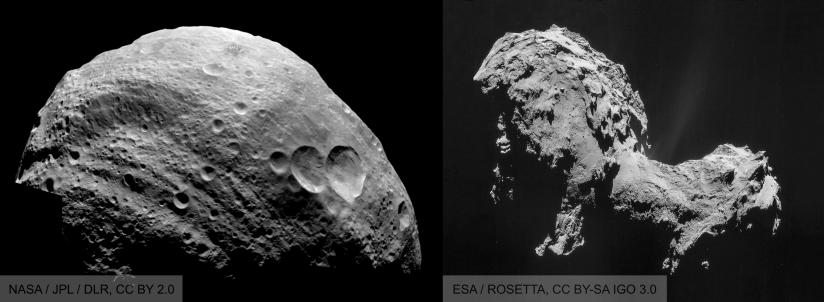
\includegraphics[width=1.0\textwidth]{images/asteroids.png}
    \caption{Photographs of 4 Vesta and 67P/Churyumov-Gerasimenko taken by the Dawn and Rosetta spacecraft, respectively (not to scale).}
    \label{fig:asteroids}
\end{figure}

In this chapter, firstly in \autoref{sec:asteroidclassification}, an overview of the various classes of asteroids will be given, based on their physical and optical properties. Afterwards, \autoref{sec:sizedistribution} will present the relation between asteroid size and frequency, as this is an important factor in determining the threat posed by asteroids. Next, in \autoref{sec:orbitalparameters} the distribution of orbital parameters of asteroids will be presented and lastly in \autoref{sec:asteroidfamilies} some major asteroid families will be discussed.

\section{Asteroid Classification}
\label{sec:asteroidclassification}

The main taxonomy of asteroids is based on the work of \cite{taxonomy}, upon which several subsequent studies have expanded. Most highly regarded, the work of \cite{smassii} aims to more precisely categorize asteroids through newly attained spectroscopic survey data, and several others such as \cite{newClassification} have further improved this process. Because the spectroscopic properties of asteroids are only a minor part of the research, the following exposition will focus on the taxonomy as proposed by Tholen. As it would be infeasible to visit every known asteroid, large-scale asteroid classification is done through spectroscopic surveys. Thus, the main classification is performed based on spectroscopic properties. \autoref{tab:asteroidclasses} gives a summary of the taxonomic classes (\cite{spectroscopicProperties}).\\
\begin{table}[htbp]
\caption{Summary of asteroid taxanomic classes.}
\label{tab:asteroidclasses}
\begin{tabular}{lll}
\textbf{Tholen Class} & \textbf{Albedo}                                                         & \textbf{Spectral Features}                                                                                                                                                                                                               \\ \hline \vspace{0.25cm}
A                     & Moderate                                                                & \begin{tabular}[c]{@{}l@{}}Very steep red slope shortward of 0.75 $\mu$m; moderately deep \\ absorption feature longward of 0.75 $\mu$m.\end{tabular}                                                        \\ \vspace{0.25cm}
B, C, F, G            & Low                                                                     & \begin{tabular}[c]{@{}l@{}}Linear, generally featureless spectra. Differences in UV absorption \\ features and presence/absence of narrow absorption feature \\ near 0.7 $\mu$m.\end{tabular}                              \\ \vspace{0.25cm}
D                     & Low                                                                     & Relatively featureless spectrum with very steep red slope.                                                                                                                                                                               \\ \vspace{0.25cm}
E, M, P               & \begin{tabular}[c]{@{}l@{}}From low (P) \\ to very high(E)\end{tabular} & \begin{tabular}[c]{@{}l@{}}Generally featureless spectrum with reddish slope; differences in \\ subtle absorption features and/or spectral curvature and/or\\  peak relative reflectance.\end{tabular}                                   \\ \vspace{0.25cm}
Q                     & Moderate                                                                & \begin{tabular}[c]{@{}l@{}}Reddish slope shortward of 0.7 $\mu$m; deep, rounded absorption \\ feature longward of 0.75 $\mu$m.\end{tabular}                                                                  \\ \vspace{0.25cm}
R                     & Moderate                                                                & \begin{tabular}[c]{@{}l@{}}Moderate reddish slope downward of 0.7 $\mu$m; deep absorption \\ longward of 0.75 $\mu$m.\end{tabular}                                                                           \\ \vspace{0.25cm}
S                     & Moderate                                                                & \begin{tabular}[c]{@{}l@{}}Moderately steep reddish slope downward of 0.7 $\mu$m; moderate to \\ steep absorption longward of 0.75 $\mu$m; \\ peak of reflectance at 0.73 $\mu$m.\end{tabular} \\ \vspace{0.25cm}
T                     & Low                                                                     & Moderately reddish shortward of 0.75 $\mu$m; flat afterwards.                                                                                                                                                              \\ \vspace{0.25cm}
V                     & Moderate                                                                & \begin{tabular}[c]{@{}l@{}}Reddish shortward of 0.7 $\mu$m; extremely deep absorption \\ longward of 0.75 $\mu$m.\end{tabular}                                                                              
\end{tabular}
\end{table}

Out of all the spectroscopic properties, the albedo is the most important parameter for the further research. Next to determining the visibility of the asteroid in sunlight, the albedo is also the main source of error in estimating the size of the target body (\cite{quantifyingrisk}). The fundamental relation which allowed for determining an asteroid's diameter from its brightness and albedo was first developed by \cite{sizealbedo} and later used by many others (e.g. \cite{populationofnea} and \cite{quantifyingrisk}). This relation is shown in \autoref{eq:sizealbedo}. Here, the brightness is given in terms of absolute magnitude $H$, diameter $D$ in km and $p_v$ representing the assumed albedo of the asteroid. For an albedo of $p_v=0.15$, this implies a diameter of $1kM$ for an object with $H=17.6$ and a diameter of $100$m for an object with $H=22.6$.

\begin{equation}
    D = \frac{1329 \mathrm{km}}{\sqrt{p_v}}10^{-H/5}
    \label{eq:sizealbedo}
\end{equation}

Because of the relation between diameter and albedo, it is important to get a reasonably accurate determination of the albedo of asteroids. Of course, because of the dependence on several unknown factors, primary among which geometry, a general estimate is to suffice. \cite{albedovalues} provides an estimate of albedo values per taxonomic class based on a numerical analysis of 84 known asteroids. This overview is shown in \autoref{tab:albedos}.\\

\begin{table}[htbp]
\centering
\caption{Mean albedo for asteroid taxonomic classes.}
\begin{tabular}{ll}
\label{tab:albedos}
\textbf{Asteroid classes} & \textbf{Mean albedo} \\ \hline \vspace{0.25cm}
C, G, B, F, P, T, D       & 0.058 $\pm$ 0.004       \\ \vspace{0.25cm}
M                         & 0.124 $\pm$ 0.009       \\ \vspace{0.25cm}
S, Q                      & 0.184 $\pm$ 0.011       \\ \vspace{0.25cm}
E, V, R                   & 0.403 $\pm$ 0.032      
\end{tabular}
\end{table}

Out of the presented classes, the C, S and V classes are most interesting for their commonality (\cite{smassiitwo}). The carbonaceous C-types make up approximately 75\% of the known asteroids, the stony S-types are the second most common at 17\% of all known asteroids. The V-type asteroid or Vestoid makes up approximately 6\% of known asteroids although they are of special interest due to their proximity to Earth and their large size, making impacts particularly dangerous (\cite{vestoid}).\\

\section{Size-Frequency Distribution}
\label{sec:sizedistribution}

Possibly the most important relation in assessing the threat of asteroid impacts is the relationship between asteroid size and frequency (\cite{firstpaper}). Whereas events such as the 2013 Chelyabinsk meteor might represent a once-in-a-decade event, globally destructive events such as the Chixculub asteroid\footnote{The asteroid popularly seen as the cause of the extinction of the non-avian dinosaurs.} might only occur once every millions of years. At this point, as Earth impacts are discussed, it is important to further constrain the selection of asteroids to those actually threatening the Earth. To this end, firstly the definition of a Near Earth Objects as used by ESA \footnote{see: \url{http://neo.ssa.esa.int/definitions-and-assumptions}} and NASA \footnote{see: \url{https://cneos.jpl.nasa.gov/about/neo_groups.html}} is given: a Near Earth Object (NEO) is an asteroid or comet with perihelion distance smaller than $1.3$AU. The vast majority of these objects are asteroids, with comets only accounting for around $1\%$ of the population. For simplicity, the description will be constrained to Near Earth Asteroids (NEA's). Among NEA's, an additional distinction exists for Potentially Hazardous Asteroids (PHA's): asteroids with a minimum orbital intersection distance of less than $0.05$AU and an absolute magnitude of 22 or less, corresponding to objects of approximately $D \geq 140$m. This last limit was determined by \cite{neosizelimit} as a balance between the difficulty of detection of smaller objects, their higher frequency, and the lower impact energy of smaller bodies. At this size, they estimated that by detecting 90\% of NEA's above this threshold, 90\% of the remaining risk over all size categories would be alleviated (\cite{subpopulations}). However, this might not be the minimal size required to properly defend planet Earth against asteroids. As \cite{smallneos} conclude, smaller objects are also worthy of study, with the Tunguska event of 1908 as an example. Objects like this, in the $30m > D > 50m$ range, "\textit{are also capable of causing significant damage to Earth... with much of the damage [of the Tunguska asteroid] caused due to shock waves from the explosion of the object in the Earth's atmosphere.}" They estimate such an event to occur once every 300 years, and advise "\textit{...to detect as many 30- to 50-meter objects as possible.}"\\

Currently, it is estimated that all NEA's with absolute magnitude $H \leq 15$ are known, corresponding to all objects of $D \geq 3.5$km at $p_v = 0.15$. To estimate the frequency of smaller asteroids, a power law was proposed by \cite{asteroidpowerlaw} which is shown in \autoref{eq:asteroidpowerlaw}. The exponent $k$, the so-called Palomar-Leiden slope, is in the range of 2.95 to 3.5 according to \cite{impactrate}. Although not entirely accurate, this relation provides a good estimate for the population of asteroids. An overview of the results of this law is given in \autoref{fig:asteroidimpact} (\cite{populationofnea}). As the impact frequency is logically an inverse function of population, and the impact energy is a linear function of mass (and therefore cubically related to diameter), these are shown as an additional reference. \\

\begin{equation}
    \frac{dN}{dD_p} \propto D_p^{-k}
    \label{eq:asteroidpowerlaw}
\end{equation}

\begin{figure}[htbp]
    \centering
    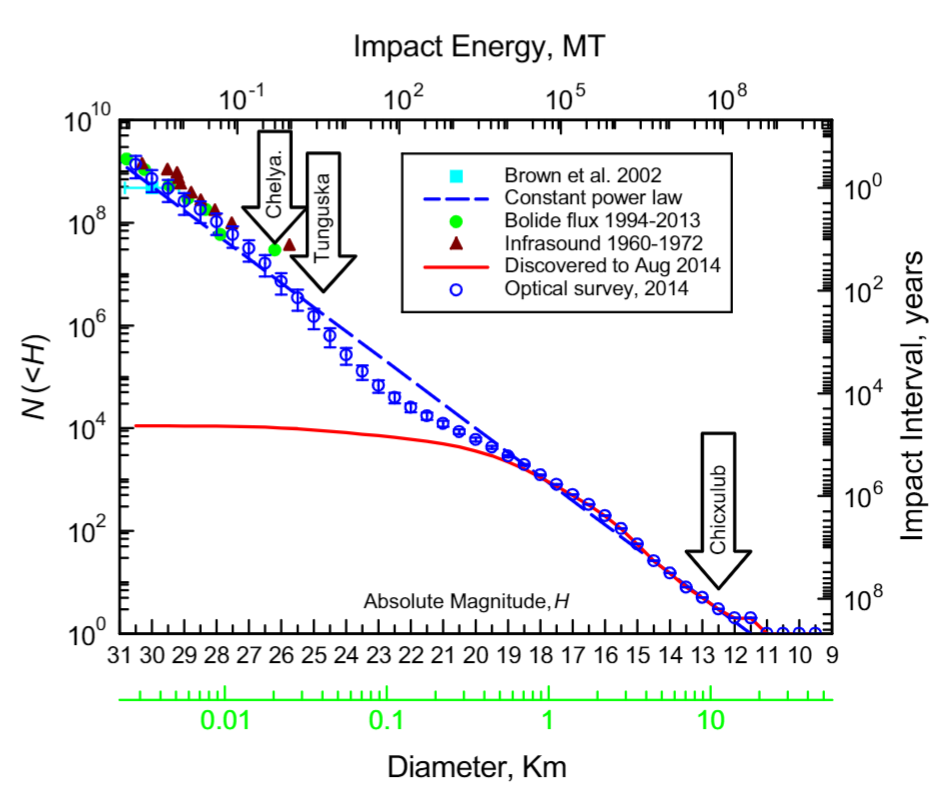
\includegraphics[width=0.68\textwidth]{images/asteroidexpectedimpact.png}
    \caption{Cumulative population, potential impact energy and impat interval for Near Earth Asteroids.}
    \label{fig:asteroidimpact}
\end{figure}

Furthermore, when assessing the feasibility of a system for asteroid detection, it should be considered which asteroids still need to be detected. As of March 2021, no objects score above a 0 ("NO HAZARD" on the Torino scale\footnote{see: \url{http://neo.ssa.esa.int/risk-page} for an overview of known NEA's with non-zero chance of impact in the next 100 years.}, therefore a potential threat will come from a currently unknown asteroid. It follows from this that the ratio of known to unknown asteroids becomes an important parameter. Frustratingly, this becomes a paradoxical problem: models of the population of asteroids are based on the asteroids we have presently detected, therefore there is no guarantee these models provide adequate information on the population of unknown asteroids. To resolve this problem, \cite{populationofnea} recently performed a numerical simulation of various distributions of orbital elements to find a distribution of orbital elements resulting in a distribution of detected objects as observed from Earth. The results are shown in \autoref{fig:asteroiddetect}. As mentioned previously, the population of asteroids of $H \leq 15$ is assumed to be near $100\%$ known. However, they also calculate that on the lower bound of NEA sizes, at $21.5 < H < 22.0$, only $6.64\%$ of NEA's is currently discovered. The full results are presented in \autoref{tab:asteroidestimation}. This fraction will get smaller as the absolute magnitude of the target body decreases, further strengthening the case for attempting to detect asteroids below the $140$m threshold. As is apparent, there are still a large number of PHA's to be discovered.

\begin{figure}[htbp]
    \centering
    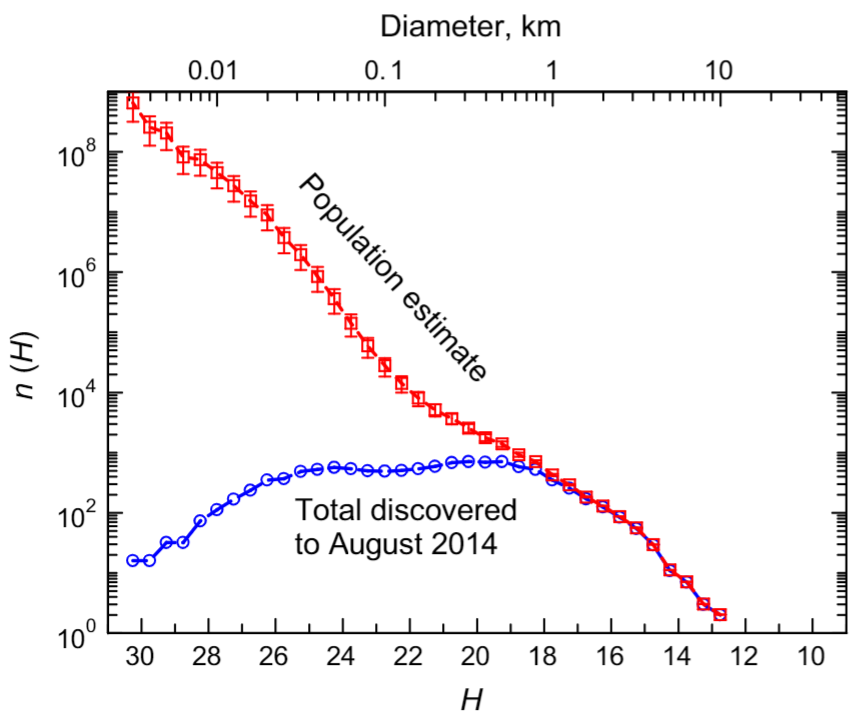
\includegraphics[width=0.6\textwidth]{images/asteroiddiscoveredexpected.png}
    \caption{Population of Near Earth Asteroids and population of those currently detected.}
    \label{fig:asteroiddetect}
\end{figure}

\begin{table}[htbp]
\centering
\caption{Estimated population and fraction discovered of NEA's by absolute magnitude}
\label{tab:asteroidestimation}
\begin{tabular}{lll}
\textbf{H range} & \textbf{Estimated population} & \textbf{Fraction discovered} \\ \hline \vspace{0.25cm}
(15.0; 15.5{]}   & 112                           & 0.978                        \\ \vspace{0.25cm}
(15.5; 16.0{]}   & 199                           & 0.969                        \\ \vspace{0.25cm}
(16.0; 16.5{]}   & 329                           & 0.953                        \\ \vspace{0.25cm}
(16.5; 17.0{]}   & 512                           & 0.927                        \\ \vspace{0.25cm}
(17.0; 17.5{]}   & 802                           & 0.886                        \\ \vspace{0.25cm}
(17.5; 18.0{]}   & 0.123E4                       & 0.826                        \\ \vspace{0.25cm}
(18.0; 18.5{]}   & 0.194E4                       & 0.740                        \\ \vspace{0.25cm}
(18.5; 19.0{]}   & 0.286E4                       & 0.631                        \\ \vspace{0.25cm}
(19.0; 19.5{]}   & 0.425E4                       & 0.509                        \\ \vspace{0.25cm}
(19.5; 20.0{]}   & 0.603E4                       & 0.387                        \\ \vspace{0.25cm}
(20.0; 20.5{]}   & 0.859E4                       & 0.276                        \\ \vspace{0.25cm}
(20.5; 21.0{]}   & 0.123E5                       & 0.185                        \\ \vspace{0.25cm}
(21.0; 21.5{]}   & 0.174E5                       & 0.115                        \\ \vspace{0.25cm}
(21.5; 22.0{]}   & 0.255E5                       & 0.664E-1                    
\end{tabular}
\end{table}

\section{Orbital Parameters}
\label{sec:orbitalparameters}

\begin{figure}[htb]
    \centering
    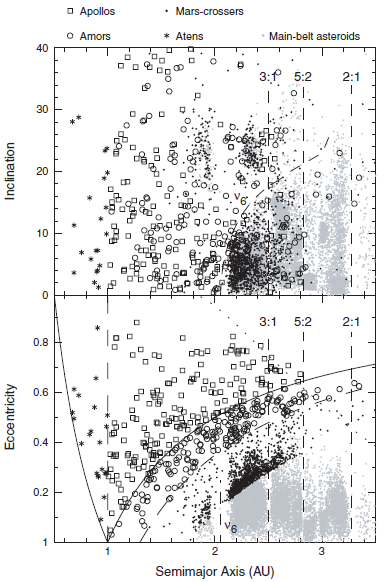
\includegraphics[width=0.5\textwidth]{images/asteroidorbits.png}
    \caption{Distribution of orbital elements of known NEO's (as of 2002) and the largest 10.000 main-belt asteroids. (\cite{originandevolution})}
    \label{fig:asteroidorbits}
\end{figure}

When discussing the hazard of asteroids, the characteristic orbits should be discussed. As can be seen in \autoref{fig:asteroidorbits}, the orbital elements are varied, but a few general conclusions can be drawn. In this section, a general overview of all NEA orbits will be given, and in \autoref{sec:asteroidfamilies} the classification will be specified into the different asteroid families. \\

The distribution of orbits can be understood better in the context of the lifecycle of near-Earth asteroids. Most near-Earth asteroid orbits are unstable on megayear timescales \cite{neonieuw}, and will eventually have their orbits altered by orbital resonances. This will lead to either impact with a planet, being launched out of the solar system by a large planet like Jupiter, or coming too close to the Sun. Because of this decay, the population has to be maintained by sources. It follows logically that over astronomical timescales a steady-state solution should be reached, which can be used as a model for the population.\\

The list of accepted primary sources for NEO's is the one presented by \cite{debiased}, further expanded upon by \cite{originandevolution}, in rough order of importance: 
\begin{itemize}
    \item The $v_6$ secular resonance between asteroids in the outer solar system and Saturn. This slows asteroids down and lowers their orbit.
    \item The 3:1 mean motion orbital resonance with Jupiter in the asteroid belt.
    \item Asteroids coming from the Intermediate Mars crosser population, being placed in near-Earth orbits by mean motion resonances with Mars, three body mean motion resonances like with Jupiter and Saturn, or other slower resonances similar to the $v_6$ resonance.
    \item Jupiter family comets, due to various gravitational interactions. However, due to their large semi-major axes and therefore long periods, this is a slow process.
    \item Outer main belt asteroids on unstable orbits in various two and three body resonances.
\end{itemize}

As might be intuitive from the variety of sources, and the evolution being driven by slow gravitational effects, the distribution of orbits is varied. An overview of known NEO's orbital distribution is shown in \autoref{fig:asteroidorbits} and \autoref{fig:phadistribution}.
Several attempts have been made at modelling the populations of NEO's based on these sources, most notably the work of \cite{debiased}, the work of \cite{subpopulations} based on the NEOWISE mission and more recently the work of \cite{neonieuw}. Some general conclusions can be drawn from this, but with some exceptions, most combinations of orbital elements are a possibility. This is important information for the further trajectory determination process.

\newpage
\begin{figure}[htb]
    \centering
    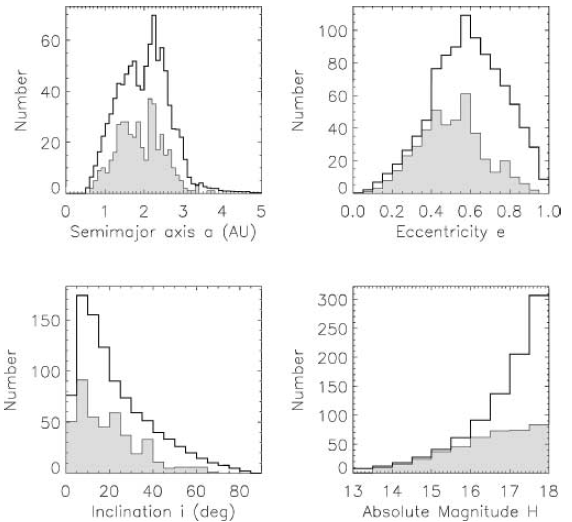
\includegraphics[width=0.7\textwidth]{images/neodist.png}
    \caption{Expected (black line) and known as of 2001 (grey histogram) distribution of orbital elements of all NEA's with H<18. (\cite{debiased})}
    \label{fig:phadistribution}
\end{figure}

\section{Major Near-Earth Asteroid Groups}
\label{sec:asteroidfamilies}

\begin{table}[htbp]
\centering
\caption{Definitions of the four main near-Earth asteroid groups.}
\label{tab:asteroidgroups}
\begin{tabular}{lllll}
\textbf{Group} & \textbf{q} & \textbf{a} & \textbf{Q} & \textbf{Earth-crossing} \\ \hline \vspace{0.25cm}
Amors          & >1.017      & >1.0        & -          & No                      \\ \vspace{0.25cm}
Apollos        & <1.017      & >1.0        & -          & Yes                     \\ \vspace{0.25cm}
Atens          & -          & <1.0        & >0.983      & Yes                     \\ \vspace{0.25cm}
Atiras         & -          & <1.0        & <0.983      & No                     
\end{tabular}
\end{table}
\newpage
\begin{figure}[htbp]
    \centering
    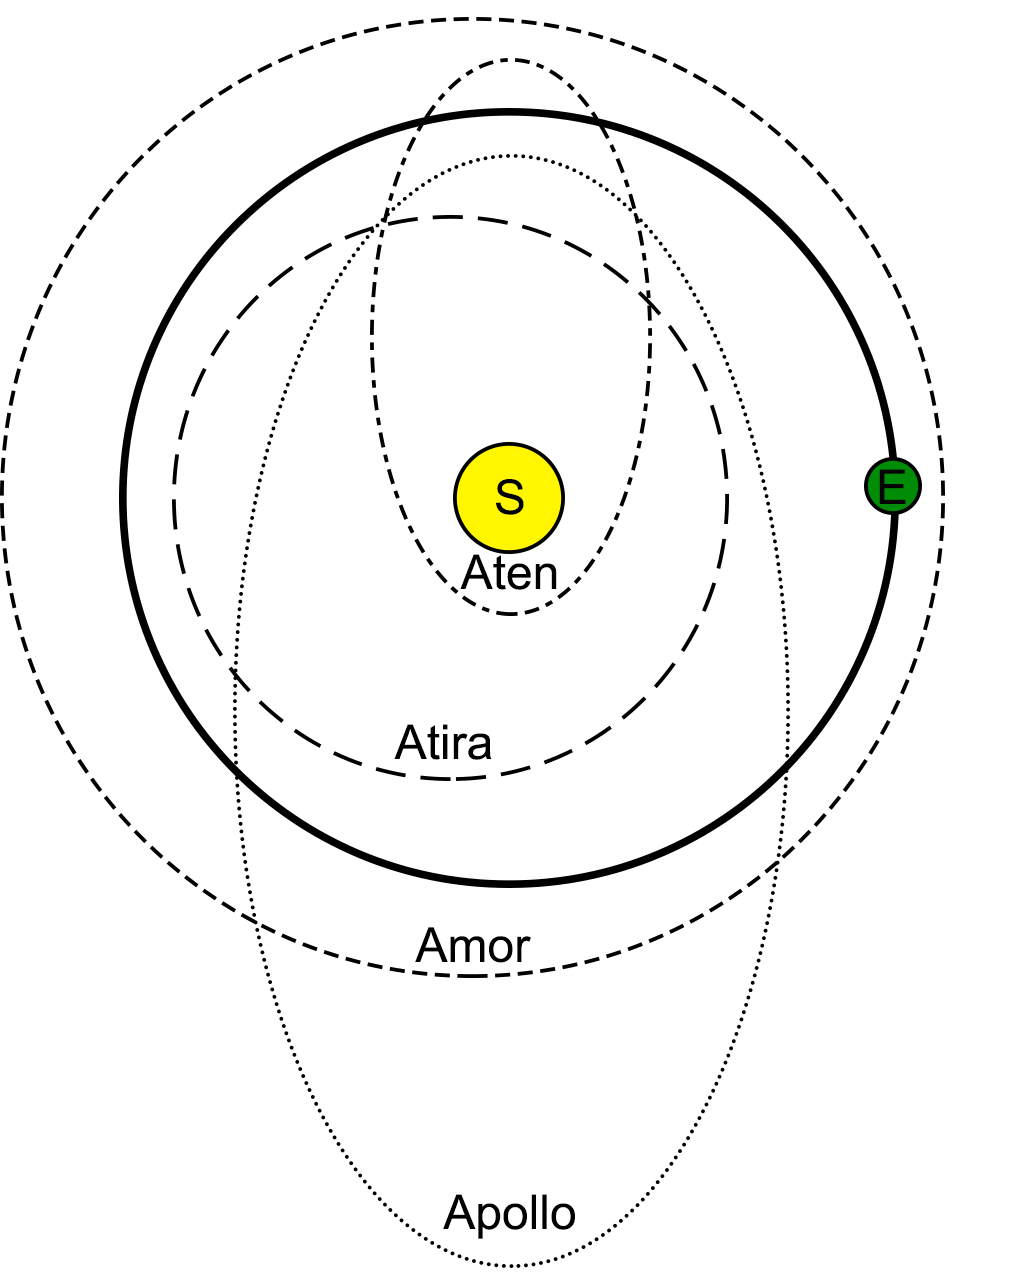
\includegraphics[width=0.4\textwidth]{images/groupdiagram.png}
    \caption{Diagram showing the characteristic orbits of the NEA groups.}
    \label{fig:neagrouporbits}
\end{figure}

To conclude the discussion of near-Earth and potentially hazardous asteroids, a cursory overview of the four main dynamical asteroid groups in the near-Earth asteroid population is presented. These groups are based on the perihelion $q$, aphelion $Q$ and semi-major axis $a$ of the asteroid's orbit. The definitions of the groups as used by NASA/JPL\footnote{see: \url{https://cneos.jpl.nasa.gov/about/neo_groups.html}} is shown in \autoref{tab:asteroidgroups} and schematically in \autoref{fig:neagrouporbits}. The boundary values for $q$ and $Q$ were chosen to coincide with the perihelion and aphelion of Earth. Although useful for reference, the Earth-crossing column does not neccessarily indicate anything about the danger of impact. As explained by \cite{dontdoECA}, the calculations involved in determining whether the asteroid will cross the orbit of Earth are laborious and error-prone. The dimensions of the orbit do not suffice: an object with a perihelion <1.0 AU and aphelion >1.0 AU is not guaranteed to intersect Earth's orbit at all; after all the orbits of asteroids can be highly inclined. \\


\newpage
\subsection{Amor Asteroids}
\begin{figure}[htb]
    \centering
    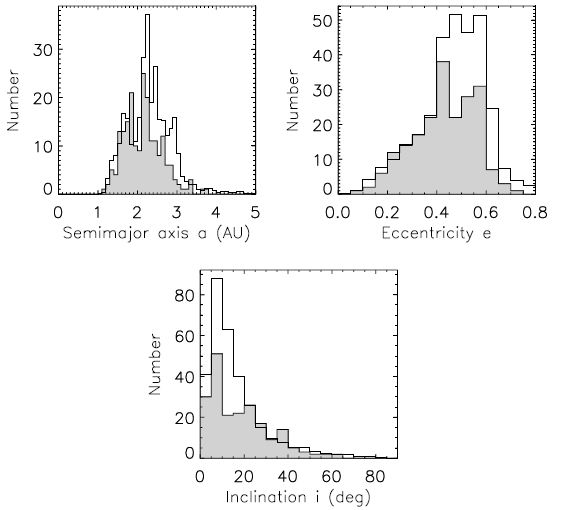
\includegraphics[width=0.7\textwidth]{images/amordist.png}
    \caption{Expected (black line) and known as of 2001 (grey histogram) distribution of orbital elements of all Amor asteroids with H<18. (\cite{debiased})}
    \label{fig:amordistribution}
\end{figure}
The Amor asteroid group features near-Earth objects conforming to the following criteria:
\begin{itemize}
    \item The semi-major axis of the objects orbit around the Sun is greater than 1.0 AU. 
    \item The perihelion is greater than Earth's aphelion.
\end{itemize}

From this follows that the orbital period is longer than one Earth year, and that the objects orbit is not Earth-crossing: the entirity of the orbit lies further away from the Sun than the orbit of Earth. The group is named after the asteroid 1221 Amor. As of March 2021, there are 9270 known Amor asteroids, of which 133 are classified as PHA\footnote{see: \url{https://ssd.jpl.nasa.gov/sbdb_query.cgi}}. The discovery fraction of the Amors is significantly higher than the other asteroid populations. This is most likely because their entire orbit is outside the orbit of Earth, and they are therefore easier to detect \cite{debiased}. Furthermore, according to results from the NEOWISE mission (\cite{subpopulations}), the Amors are proportionally dark, with $35\%$ of the population having $p_v < 0.01$. Their size distribution can be fit to \autoref{eq:asteroidpowerlaw} using $k = 1.40\pm0.18$ for asteroids with $D<1.9\mathrm{km}$ and $k=5.0\pm2.0$ for larger sizes. The distribution of orbital parameters is shown in \autoref{fig:amordistribution}.

\newpage
\subsection{Apollo Asteroids}
\begin{figure}[htb]
    \centering
    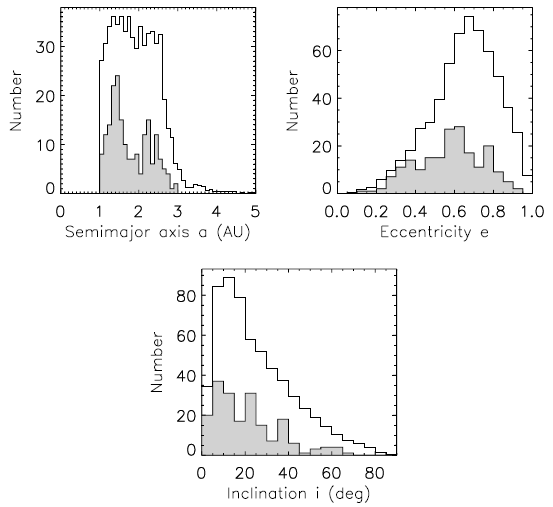
\includegraphics[width=0.7\textwidth]{images/apollodist.png}
    \caption{Expected (black line) and known as of 2001 (grey histogram) distribution of orbital elements of all Apollo asteroids with H<18.(\cite{debiased})}
    \label{fig:apollodistribution}
\end{figure}
The Apollo asteroid group features near-Earth objects conforming to the following criteria:
\begin{itemize}
    \item The semi-major axis of the objects orbit around the Sun is greater than 1.0 AU.
    \item The perihelion is smaller than Earth's aphelion.
\end{itemize}

Like the Amor asteroids, this gives the Apollos an orbital period of greater than one year. Because of their lower perihelion, the Apollos are Earth-crossing. The group is named after 1862 Apollo. As of March 2021, there are 14013 known Apollo asteroids, of which 1836 are classified as PHA\footnote{see: \url{https://ssd.jpl.nasa.gov/sbdb_query.cgi}}. The discovery fraction of Apollos is smaller than the Amors and Atens. This is possibly because their higher eccentricity makes the Apollos have a larger velocity when passing near Earth. This makes them harder to detect. This is supplemented by the fact that especially in the higher eccentricities or inclinations, there are less Apollos detected than expected \cite{debiased}. The Apollos are slightly less dark than the Amors, with $30\%$ of the population having $p_v < 0.09$. Furthermore, their size distribution can be modeled with $k = 1.44\pm0.12$ for objects with $D<1.6\mathrm{km}$ and $k=3.0\pm1.5$ for $D>1.6\mathrm{km}$\cite{subpopulations}. The distribution of orbital parameters is shown in \autoref{fig:apollodistribution}. The asteroid which exploded over Chelyabinsk, Russia in 2013 was an Apollo asteroid.

\newpage
\subsection{Aten Asteroids}
\begin{figure}[htb]
    \centering
    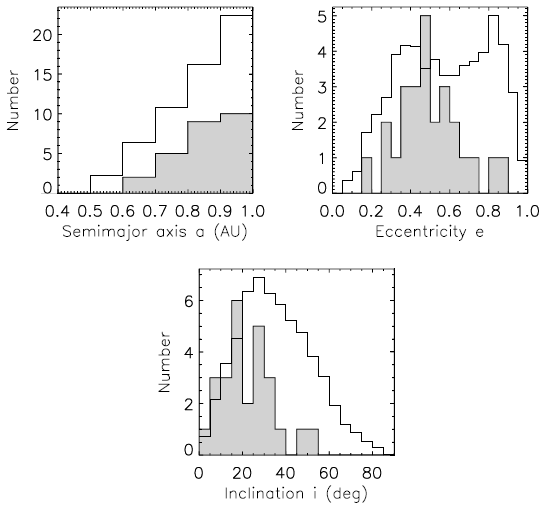
\includegraphics[width=0.7\textwidth]{images/atendist.png}
    \caption{Expected (black line) and known as of 2001 (grey histogram) distribution of orbital elements of all Aten asteroids with H<18. (\cite{debiased})}
    \label{fig:atendistribution}
\end{figure}

The Aten asteroid group features near-Earth objects conforming to the following criteria:
\begin{itemize}
    \item The semi-major axis of the objects orbit around the Sun is smaller than 1.0 AU.
    \item The aphelion is greater than Earth's perihelion.
\end{itemize}

This gives the Aten asteroids an orbital period less than a year, and makes their orbits Earth-crossing. The group is named after 2062 Aten. As of March 2021, there are 1935 known Aten asteroids, of which 174 are classified as PHA\footnote{see: \url{https://ssd.jpl.nasa.gov/sbdb_query.cgi}}. The discovery fraction of the Atens is quite good, owing to their lower velocity than the Apollos, and the fact that, due to their lower semi-major axis, they can not be far away from Earth at opposition \cite{debiased}. The Atens are a bright group, with only $17\%$ of the population having $p_v < 0.09$. Their size distribution can be modelled using \autoref{eq:asteroidpowerlaw} with $k = 1.63\pm0.30$. \cite{subpopulations} The distribution of orbital parameters is shown in \autoref{fig:atendistribution}. The asteroid 99942 Apophis, which briefly caused a scare in 2004 because of a rumored impact trajectory, is an Aten asteroid.

\newpage
\subsection{Atira Asteroids}
\begin{figure}[htb]
    \centering
    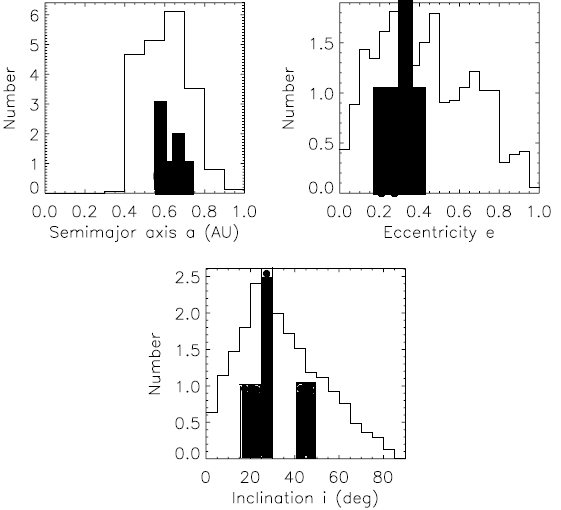
\includegraphics[width=0.7\textwidth]{images/atiradist.png}
    \caption{Expected (black line) and known as of 2020 (black histogram) distribution of orbital elements of all Atira asteroids with H<18.(\cite{debiased}). The black histogram was not presented in the original paper, but was added by the author of this report. This was done because there were zero known Atira asteroids in 2001. Note that there is still a lot of uncertainty in this population.}
    \label{fig:atiradistribution}
\end{figure}

The Atira asteroids, sometimes also refered to as Apohele asteroids or interior-Earth objects, are near-Earth objects conforming to the following criteria:
\begin{itemize}
    \item The semi-major axis of the objects orbit around the Sun is smaller than 1.0 AU.
    \item The aphelion is smaller than Earth's perihelion.
\end{itemize}

Similar to the Aten asteroids, the Atira asteroids feature an orbital period shorter than one year. Because of their characteristics, their orbits are entirely contained within Earth's orbit. The group was named after the first confirmed member, 163693 Atira. The Atira's are by far the smallest group, with, as of March 2021, only 23 known objects, of which 6 classified as PHA\footnote{see: \url{https://ssd.jpl.nasa.gov/sbdb_query.cgi}}/ Although it should not be impossible to detect Atira asteroids, their observation is more challenging. A simple geometric calculation will show that the Atira asteroids can be viewed at phase angles around $70^\circ$. However, as most detections are serendipitous and the population is expected to be small, there are very few known Atira asteroids. \cite{debiased}. Therefore, additional information is scarce. The expected distribution of orbital parameters is shown in \autoref{fig:atiradistribution}.